\section{Cachipún}

Escriba un programa para jugar cachipún contra el computador. La
interfaz debe ser la siguiente:

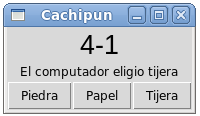
\includegraphics{../../diapos/programas/tkinter/capturas/16.png}

Cada vez que usted haga clic en un botón, el computador debe elegir al
azar su jugada (piedra, papel o tijera), y mostrarla en la etiqueta («El
computador eligió\ldots{}»). Además, hay que actualizar el marcador que
indica cuántas veces ha ganado cada uno. En el ejemplo de la imagen, el
humano ha ganado cuatro veces, y el computador una.

La regla para saber quién ganó es: piedra le gana a tijera, tijera le
gana a papel, papel le gana a piedra. El resto de las combinaciones
posibles son todas empates.
